\chapter{State Of The Art}

\section{Introduction}
In this section, we discuss most popular search and indexing engines and their advantages and disadvantages.
 

\section{Indexing}

indexing is a mechanism to optimize the performance of a database by minimizing the number of disk accesses required when a query is processed. \\
It is a data structure technique which is used to quickly locate and access the data in a database.\\
An Index is a small table having only two columns.
\begin{itemize}
    \item The first  column comprises a copy of the primary or candidate key of a table.
    \item The second column contains a set of pointers for holding the address of the disk block where that specific key value stored.
\end{itemize}

\section{Apache Lucene}
\subsection{What is Lucene ?}
Apache Lucene is a high-performance, scalable information retrieval ( IR ) library. IR refers to
the process of searching for documents, information within documents, or metadata
about documents.

\subsection{Apache Lucene Features}
Lucene provides search over documents; where a document is essentially a collection of fields. 
A field consists of a field name that is a string and one or more field values.
Lucene does not in any way constrain document structures. Fields are constrained to store only one kind of data, either binary, numeric, or text data. There are two ways to store text data.\\
Lucene provides many ways to break a piece of text into tokens as well as hooks that allow you to write custom tokenizers. Lucene has a highly expressive search API that takes a search query and returns a set of documents ranked by relevancy with documents most similar to the query having the highest score.\\
In a nutshell, the features of Lucene can be described as follows:
\subsubsection{Scalable and High-Performance Indexing}
\begin{itemize}
    \item Small RAM requirements.
    \item Incremental indexing as fast as batch indexing.
    \item Index size roughly 20-30\% the size of text indexed.
\end{itemize}

\subsubsection{Powerful, Accurate, and Efficient Search Algorithms}
\begin{itemize}
    \item Provides Ranked search
    \item Supports many powerful query types: phrase queries, wildcard queries, proximity queries, range queries and more.
    \item Provides fielded searching.
    \item Supports multiple-index searching with merged results.
    \item It allows simultaneous update and searching.
    \item Supports sorting by any field.
\end{itemize}

\subsubsection{Cross-platform solution}
\begin{itemize}
    \item Available as Open Source software.
    \item It is 100\%-pure Java.
\end{itemize}

\subsection{How Does Apache Lucene Work?}
In this Section, we will discuss how does Apache Lucene work towards indexing and searching. 
\subsubsection{Using Inverted Index}
Lucene stores it's input into a data structure called inverted index .This data structure makes
efficient use of disk space while allowing quick keyword lookups.\\
What makes this structure inverted is that it uses tokens extracted from input documents as lookup keys
instead of treating documents as the central entities. In other words, rather than
trying to answer the question “What words are contained in this document?” this struc-
ture is optimized for providing quick answers to “Which documents contain word X ?”.
\subsubsection{Document Indexing}
Document indexing consists of first constructing a document that contains the fields to be indexed or stored, then adding that document to the index.
Every Lucene Index consists of one or more segments, as depicted in .\\
Each segment is a standalone index, holding a subset of all indexed documents.
\\
\\
\\
\begin{figure}[!htb]
\begin{center}
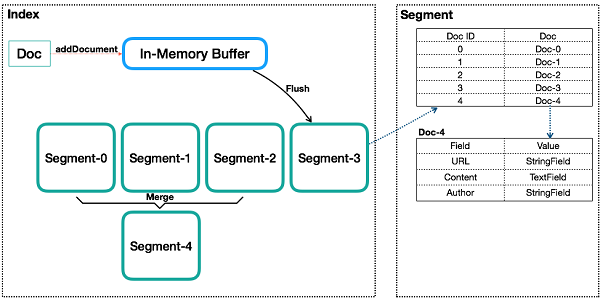
\includegraphics[scale=1.0]{images/segments.png}
\end{center}
\caption[Analysis of Lucene - Basic Concepts]{The figure shows the basic internal structure of an index. The data in a segment is represented abstractly rather than as a realistic representation of the actual data structure.}
\label{lucene_segments}
\end{figure}

\section{Search Engines}
In this section, we present the most popular open-source search engines and make a comparison of them in order to find the one who fits our need. 

\subsection{Elasticsearch}
Elasticsearch is highly scalable open-source search and analytics engine.it provides a distributed
system on top of Apache Lucene for indexing and automatic type guessing and utilizes a JSON based REST API which make it easy to our application to communicate with ES.
On top of Lucene functionalities ES adds its own:
\begin{itemize}
    \item Query Caching
    \item Real-Time Analytics
    \item Fully Distributed Model
\end{itemize}

\subsubsection{Easy To Use}
It is easy to set up out of the box since it ships with sensible defaults and hides complexity from beginners. 
It has a short learning curve to grasp the basics so anyone with a bit of efforts can become productive very quickly. It is schema-less, using some defaults to index the data.

\subsubsection{One Trick JSON Format}
Since ES exposes a REST API to index and search data. its not possible to use other data format such as pdf, xml and csv. So, in order to index these format
we need to use third-party plugins.

\subsection{Apache Solr}
Like ES, Apache Solr is an open-source search engine built on top of Apache Lucene. It provides a scalable enterprise wide search capability for a diverse set of data types including: NoSQL, rich document (PDF/Binary/MS-Word), relational database, and more. Features include faceted search, hit highlighting, full-text search. It was designed for scale and fault tolerance.

\subsubsection{Data Sources}
Solr accept data from different sources including XML files, comma-separated value (CSV) files, and data extracted from tables in a database as well as common file formats such as Microsoft Word and PDF.

\subsubsection{Searching}
With the variety of analyzers and tokenizers implemented in Apache Solr. It is much more oriented towards full-text search.\\
While ES is often used for analytical querying, filtering, and grouping.

\subsubsection{Cloud Environnement}
Apache Solr - in its Elasticsearch-like fully distributed SolrCloud deployment mode - depends on Apache ZooKeeper. 
Although ZooKeeper is mature and widely used, it’s ultimately an entirely separate application. SolrCloud is designed to provide a highly available, fault-tolerant environment for distributing indexed content and query requests across multiple servers. With SolrCloud, data is organized into multiple pieces that can be hosted on multiple machines. The replicas will help to achieve redundancy as well as scalability and fault-tolerance.

\subsection{Sphinx}
Sphinx is open source search engine. Sphinx allow full-text searches. Sphinx is very efficient to perform search over large data. Sphinx can index data from various different sources like: MySQL, HTML, Text Files etc.

\subsubsection{Data Sources}
From Sphinx point of view, the data it indexes is a set of structured documents, each of which has the same set of fields and attributes. 
This is similar to SQL, where each row would correspond to a document, and each column to either a field or an attribute.

\subsubsection{Distributed Mode}
In Order to make Sphinx run in distributed mode. We need to do partitioning by hand, then create special distributed index on some of the Sphinx instances. 
In distributed mode we can't achieve replication with Sphinx.

\section{Conclusion}
The main aim of this project is to:
\begin{itemize}
    \item Index Investment Data
    \item Provide Descriptive Analysis
\end{itemize}
Then, we must consider analytics and visualizations a core component of our use cases.
So we choose Elasticsearch as search and indexing engine for our framework because of his simplicity, quering features 
and capability to scale.